\begin{figure}
\centering
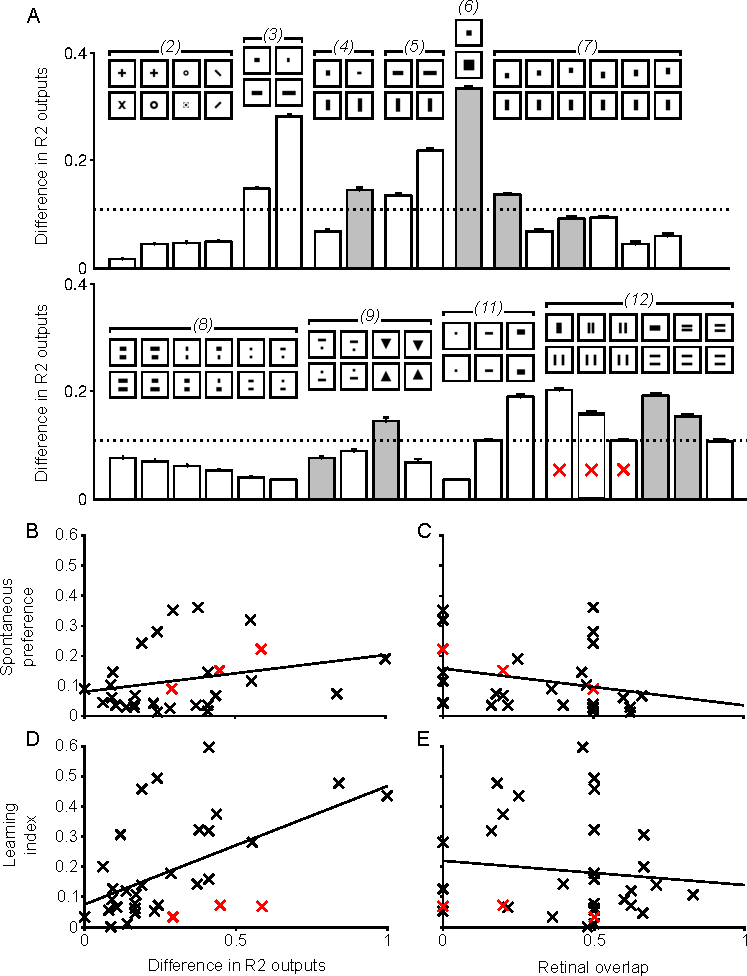
\includegraphics{figures/pattern}
\caption{How discriminable are different patterns for R2 neurons?
The bars indicate the \ac{rms} difference in activation for the R2 neurons when a pattern is at a rotation of 0\degree\ and 90\degree.
A lower score indicates that the fly should find the pattern more difficult to discriminate.
Error bars show the standard error over the whole \ac{RIDF} (for examples see Figure~\ref{fig:recap}C--F).
The patterns are drawn from \protect\cite{Ernst1999}; only patterns for which a statistical test was performed on the `differential conditioned preference' index ($\overline{\mathrm{DCP}}$) are included.
Where the $\overline{\mathrm{DCP}}$ score for a given pattern was significant in \protect\cite{Ernst1999}, the degree of significance is indicated by asterisks adjacent to the bars.
}
\label{fig:pattern}
\end{figure}
